\documentclass[12pt,a4paper,openany]{extarticle}
% подключаем собственный стилевой файл
\usepackage{mystyle}
\selectlanguage{russian}
\graphicspath{{./pictures/}}
\usepackage[pdftex]{lscape}
\usepackage{graphicx}
\usepackage{systeme}

\begin{document}
\part*{Лабораторная работа №2\\ Идентификация трения. Расчет коэффициентов регуляторов.}%Трения чего?
\section{Методические рекомендации}
\hspace*{\parindent}До начала работы студент должен выполнить предыдущие лабораторные этого цикла.%пред. семестр

\section{Теоретические сведения}

\paragraph*{Математическая модель сочленения\\}
\hspace*{\parindent} Одномерное управление вращательным сочленением фактически сводится к управлению двигателем постоянного тока с зубчатой передачей, динамическая модель которого содержит две составляющие: электрическую и механическую. Рассмотрим их математическое описание.

Электрическая компонента, обусловленная электрической цепью из индуктивности, резистора и двигателя, определяется выражением:
\begin{equation}\label{1}
	L\dot{i}(t)+Ri(t)=u(t)-K_e\dot{\theta}(t),
\end{equation}
где $L, R, i(t), u(t)$ - индуктивность, сопротивление, сила тока и напряжение якоря, соответственно, $K_e$ - коэффициент противо-ЭДС, $\theta(t), \dot{\theta}(t) $ -  угловая скорость и угол поворота ротора, соответственно.

Механическая  компонента,  обусловленная  зубчатой  передачей,определяется выражением:
\begin{equation}\label{2}
	 J_m\ddot{\theta}(t)+K_f\dot{\theta}(t)=K_mi(t) - \mu_l(t),
\end{equation}
где $J_m$ -  приведенный момент инерции, $K_f, K_m$ - коэффициент трения и коэффициент момента силы соответственно, $\mu_l(t) $ - момент нагрузки, $\ddot{\theta}(t) $ - угловое ускорение ротора.

\paragraph*{Преобразование Лапласа и передаточная функция\\}
\hspace*{\parindent} Преобразованием Лапласа функции вещественной переменной $f(t)$ называется функция $F(s)$ комплексной переменной $s=\sigma+i\omega$ такая, что:
\begin{equation}
	F(s) = \mathcal{L}\{f(t)\} = \int\limits_{0}^{\infty} e^{-st}f(t)dt.
\end{equation}
Функцию $f(t)$ называют оригиналом, а функцию $F(s)$ - изображением функции $f(t)$.

Особенностью преобразования Лапласа является то, что многим соотношениям и операциям над оригиналами соответствуют более простые соотношения над их изображениями. 

Например, изображением производной от оригинала является произведение изображения оригинала на $s$ за вычетом значения оригинала при $t=0$:
\begin{equation}
	\mathcal{L}\{f'(t)\} = sF(s) - f(0),
\end{equation}
а изображением интеграла от оригинала является изображение оригинала, деленное на $s$:
\begin{equation}
	\mathcal{L}\{\int_{0}^{x} f(t)dt\}=\frac{F(s)}{s}.
\end{equation}
Так же, преобразование Лапласа обладает свойством линейности:
\begin{equation}
	\mathcal{L}\{af(t)+bg(t)\}=aF(s)+bG(s).
\end{equation}

Передаточной функцией $W(s)$ называется отношение преобразования Лапласа выходного сигнала к преобразованию Лапласа входного сигнала при нулевых начальных условиях:
\begin{equation}
	W(s) = \frac{Y(s)}{U(s)}.
\end{equation}

Найдем передаточную функцию сочленения. Для этого, осуществим преобразование Лапласа функций \eqref{1} и \eqref{2}, выполним структурные преобразования и получим:
\begin{equation}
	\left\{	
		\begin{aligned}
			&LsI(s)+RI(s)=U(s)-K_es\Theta(s)\\
			&J_ms^2\Theta(s) + K_fs\Theta(s) = K_mI(s) - M_l(s)
		\end{aligned}
	\right.
\end{equation}
\begin{equation}
	\left\{	
		\begin{aligned}
			&(Ls+R)I(s)=U(s)-K_es\Theta(s)\\
			&(J_ms + K_f)s\Theta(s) = K_mI(s) - M_l(s)
		\end{aligned}
	\right.
\end{equation}
\begin{equation}
	\left\{	
		\begin{aligned}
			&I(s)=\frac{U(s)-K_es\Theta(s)}{Ls+R}\\
			&(J_ms + K_f)s\Theta(s) = K_mI(s) - M_l(s)
		\end{aligned}
	\right.
\end{equation}
\begin{equation}
	(Js+K_f+\frac{K_eK_m}{Ls+R})s\Theta(s)=\frac{K_mU(s)}{Ls+R}-M_l(s)
\end{equation}
\begin{equation}\label{lap}
	\Theta(s) = \frac{K_mU(s)-M_l(s)(Ls+R)}{s((Ls+R)(J_ms+K_f)+K_eK_m)}
\end{equation}
Затем, из \eqref{lap} запишем передаточную функцию от входа $U(s)$ к выходу $\Theta(s)$ при $M_l(s) = 0$:
\begin{equation}\label{OU}
	\frac{\Theta(s)}{U(s)}=\frac{K_m}{s((Ls+R)(J_ms+K_f)+K_eK_m)}.
\end{equation}
Передаточная функция от $M_l(s)$ к $\Theta(s)$ при $U(s) = 0$: 
\begin{equation}\label{OM}
	\frac{\Theta(s)}{M_l(s)}=-\frac{Ls+R}{s((Ls+R)(J_ms+K_f)+K_eK_m)}.
\end{equation}
Разделим числитель и знаменатель передаточных функций \eqref{OU} и \eqref{OM} на $R$:
\begin{equation}\label{OUR}
	\frac{\Theta(s)}{U(s)}=\frac{\frac{K_m}{R}}{s((\frac{L}{R}s+1)(J_ms+K_f)+\frac{K_eK_m}{R})},
\end{equation}
\begin{equation}\label{OMR}
	\frac{\Theta(s)}{M_l(s)}=-\frac{\frac{L}{R}s+1}{s((\frac{L}{R}s+1)(J_ms+K_f)+\frac{K_eK_m}{R})}.
\end{equation}
Допуская, что постоянная времени электрической компоненты существенно меньше, чем постоянная времени механической части:
\begin{equation}
	\frac{L}{R}\ll\frac{J}{k_f},
\end{equation}
что является типичным допущением для электромеханических частей, перепишем передаточные функции \eqref{OUR} и \eqref{OMR}:
\begin{equation}\label{OUR2}
	\frac{\Theta(s)}{U(s)}\approx\frac{\frac{K_m}{R}}{s(J_ms+K_f+\frac{K_eK_m}{R})},
\end{equation}
\begin{equation}\label{OMR2}
	\frac{\Theta(s)}{M_l(s)}\approx-\frac{1}{s(J_ms+K_f+\frac{K_eK_m}{R})}.
\end{equation}
Введем новые обозначения и упростим передаточные функции \eqref{OUR2} и \eqref{OMR2}:
\begin{equation}\label{OUR3}
	\frac{\Theta(s)}{M_u(s)}\approx\frac{1}{s(J_ms+K)},
\end{equation}
\begin{equation}\label{OMR3}
	\frac{\Theta(s)}{M_l(s)}\approx-\frac{1}{s(J_ms+K)}.
\end{equation}
где $M_u(s)= \frac{K_m}{R}U(s)$, $K=K_f+\frac{K_eK_m}{R}$.
Комбинируя передаточные функции \eqref{OUR3} и \eqref{OMR3}, при $U(s)\neq0$ и $M_l(s)\neq0$ получим:
\begin{equation}\label{pfunction}
	\Theta(s)=\frac{1}{s(J_ms+K)}(M_u(s)-M_l(s))=P(s)(M_u(s)-M_l(s)).
\end{equation}

Таким образом, мы получили математическую модель вращательного сочленения в виде передаточной функции $P(s)$. Из этой функции можно получить дифференциальное уравнение системы. Для этого разделим обе части \eqref{pfunction} на $P(s)$:
\begin{equation}
	J_ms^2\Theta(s)+Ks\Theta=M_u(s)-M_l(s),
\end{equation}
осуществим обратное преобразование Лапласа:
\begin{equation}
	J_m\ddot{\theta}(t)+K\dot{\theta}(t)=\mu_u(t)-\mu_l(t),
\end{equation}
разделим на $J_m$ и вернем старые обозначения:
\begin{equation}\label{dif}
	\ddot{\theta}(t)+(\frac{K_f}{J_m}+\frac{K_eK_m}{J_mR})\dot{\theta}(t)=\frac{K_m}{J_mR}u(t)-\frac{\mu_l(t)}{J_m}.
\end{equation}
\paragraph*{Идентификация трения\\}%Трения чего?
\hspace*{\parindent}В предыдущих лабораторных работах были найдены параметры $J_m^1, K_e^1, K_m^1, R$ для мотора NXT. В данной лабораторной работе исследуется сочленение манипулятора, коэффициент редукции которого отличается от коэффициента мотора NXT в $i$ раз. Для нахождения новых значений параметров $J_m, K_e, K_m$ нужно вычислить значение коэффициента редукции $i$, разделив количество зубьев ведомой шестерни на количество зубьев ведущей. Затем, рассчитать новые параметры по формулам:
\begin{equation}
	J_m=J_m^1i^2, \phantom{-} K_e = K_e^1i, \phantom{-} K_m = K_m^1i,
\end{equation}

Для нахождения значения коэффициента трения воспользуемся методом наименьших квадратов. На вход системы будем подавать напряжение $u(t) = U_m\sin{{\omega}t}$, где $U_m$ - максимальное напряжение двигателя. Для аппроксимации функции необходимо решить дифференциальное уравнение \eqref{dif}. Его решением будет следующая функция:
\begin{equation}\label{theta}
	\theta(t)=\frac{B(A^2(1-\cos{{\omega}}t)+\omega^2(1-e^{-At})-A\omega\sin{{\omega}t)}}{A\omega(A^2+\omega^2)},
\end{equation}где $A=\frac{K_f}{J_m}+\frac{K_eK_m}{J_mR}$, $B=\frac{K_mU_m}{J_mR}$.

Считая $K_f = 0$, рассчитаем значения $A$ и $B$ и построим график при $u(t) = U_m\sin{2t}$, изображенный на рис.~\ref{nofr}.

\begin{figure}[h]
	\noindent\centering{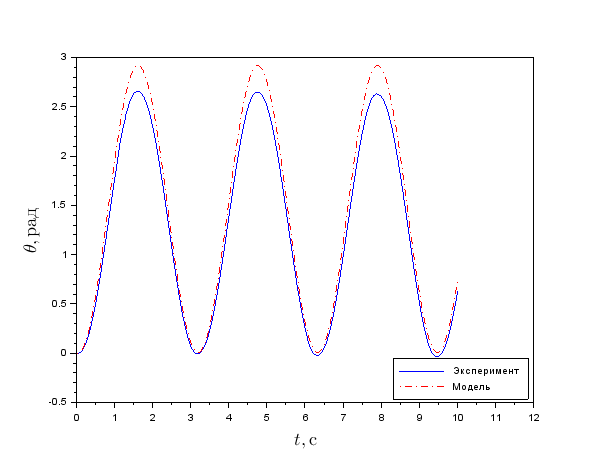
\includegraphics[height = 6cm]{img/sin2.png}}
	\caption{График модели без учета трения}
	\label{nofr}
\end{figure}

Аппроксимируем функцию \eqref{theta} по $A$ с помощью функции "datafit" пакета \textit{Scilab} и построим график, изображенный на рис.~ \ref{yesfr}. Так как $A$ зависит от неизвестного коэффициента $K_f$, то аппроксимирую функцию по $A$ мы учитываем $K_f$. %можем найти K_f

\begin{figure}[h]
	\noindent\centering{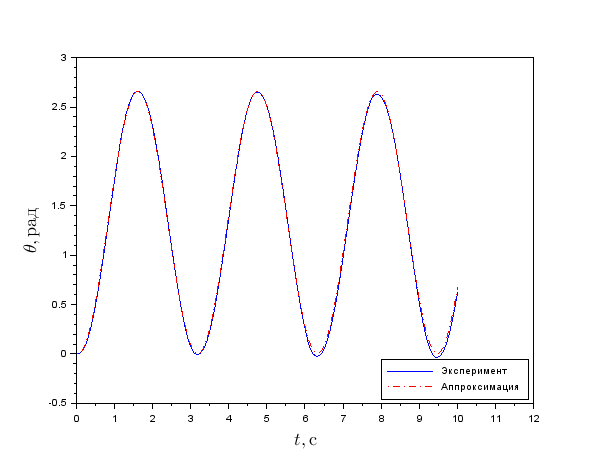
\includegraphics[height = 6cm]{img/kfsin2.png}}
	\caption{График модели с учетом трения}
	\label{yesfr}
\end{figure}

Очевидно, что введение коэффициента $K_f$ сделало математическую модель двигателя более правдоподобной.

Из полученного значения $A$ выведем:
\begin{equation}
	K_f = J_mA-\frac{K_eK_m}{R}, \phantom{-} K=J_mA,
\end{equation}

% Для чего учет трения
\paragraph*{ПИД-регулятор угла поворота\\}
\hspace*{\parindent}Введем пропорционально-интегрально-дифференциальный (ПИД) регулятор с передаточной функцией $R(s)$:
\begin{equation}
	R(s)=k_p+k_i\frac{1}{s}+k_ds.
\end{equation}
На рис.~\ref{pid} изображена схема моделирования системы с таким регулятором.

\begin{figure}[h]
	\noindent\centering{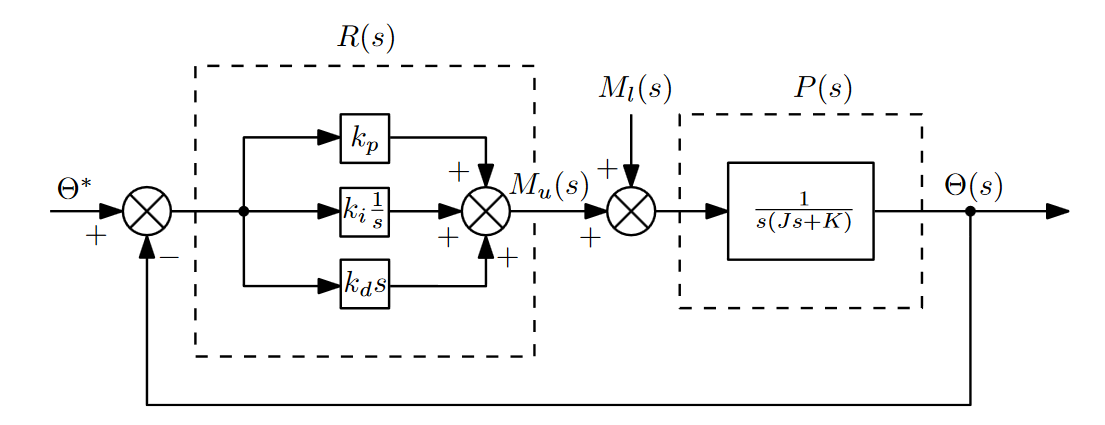
\includegraphics[height = 6cm]{img/mod.png}}
	\caption{Схема моделирования системы с ПИД-регулятором}
	\label{pid}
\end{figure}

\hspace*{\parindent}Выразим из нее выходную переменную:
\begin{equation}
	\Theta(s)=(\Theta^*(s)-\Theta(s))R(s)P(s)-M_l(s))P(s),
\end{equation}
\begin{equation}
	\Theta(s)+\Theta(s)R(s)P(s)=\Theta^*R(s)P(s)-M_l(s)P(s),
\end{equation}
\begin{equation}
	\Theta(s)=\frac{R(s)P(s)}{1+R(s)P(s)}\Theta^*(s)-\frac{P(s)}{1+R(s)P(s)}M_l(s),
\end{equation}
где $\Theta^*(s)$ - желаемый угол поворота.

Рассчитаем передаточную функцию системы при $M_l(s)=0$:
\begin{equation}\label{pidfunc}
	W(s)=\frac{\Theta(s)}{\Theta^*(s)}=\frac{R(s)P(s)}{1+R(s)P(s)}=\frac{\frac{k_ds^2+k_ps+k_i}{J_ms^3+Ks^2}}{1+\frac{k_ds^2+k_ps+k_i}{J_ms^3+Ks^2}}=\frac{k_ds^2+k_ps+k_i}{J_ms^3+(K+k_d)s^2+k_ps+k_i}
\end{equation}

Корни полинома в числителе передаточной функции называются нулями, а корни полинома в знаменателе – полюсами. Знаменатель передаточной функции является характеристическим полиномом дифференциального уравнения движения системы. На основании корней характеристического полинома $J_ms^3+(K+k_d)s^2+k_ps+k_i$ передаточной функции \eqref{pidfunc}, зная значения $J_m$ и $K$,  можно рассчитать такие коэффициенты ПИД-регулятора, чтобы обеспечивались требуемые показатели качества системы. 

\paragraph*{ПИ-регулятор угловой скорости\\}
\hspace*{\parindent}Аналогично, можно вывести регулятор угловой скорости. Сначала, из \eqref{pfunction} получим функцию для угловой скорости:
\begin{equation}
	\Omega(s)=s\Theta(s)=\frac{1}{J_ms+K}(M_u(s)-M_l(s))=P^1(s)(M_u(s)-M_l(s))
\end{equation}

\begin{figure}[h]
	\noindent\centering{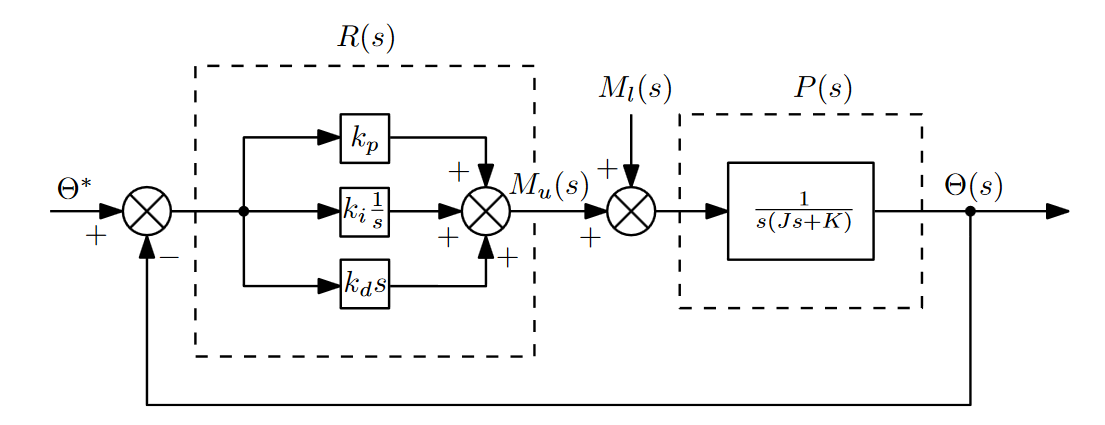
\includegraphics[height = 6cm]{img/mod2.png}}
	\caption{Схема моделирования системы с ПИ-регулятором}
	\label{pi}
\end{figure}

Введем ПИ-регулятор с передаточной функцией:
\begin{equation}
	R^1(s)=k_p^1+k_i^1\frac{1}{s}
\end{equation}
На рис.~\ref{pi} изображена схема моделирования системы с таким регулятором.

Аналогично \eqref{pidfunc}, получим передаточную функцию системы:
\begin{equation}\label{pifunc}
	W^1(s)=\frac{\Omega(s)}{\Omega(s)^*}=\frac{R^1(s)P^1(s)}{1+R^1(s)P^1(s)}=\frac{\frac{k_p^1s+k_i^1}{J_ms^2+Ks}}{1+\frac{k_p^1s+k_i^1}{J_ms^2+Ks}}=\frac{k_p^1s+k_i^1}{J_ms^2+(K+k_p^1)s+k_i^1},
\end{equation}
где $\Omega^*(s)$ - желаемая скорость поворота.

На основании корней характеристического полинома $J_ms^2+(K+k_p^1)s+k_i^1$ передаточной функции \eqref{pifunc} можно рассчитать такие коэффициенты ПИ-регулятора, чтобы обеспечивались требуемые показатели качества системы. Рассмотрим, как это можно сделать. 
\paragraph*{Устойчивость системы\\}
\hspace*{\parindent}Система называется устойчивой, если после снятия внешнего возмущения она возвращается в исходное состояние. Так как движение системы в свободном состоянии описывается однородным дифференциальным уравнением, то математическое определение устойчивой системы можно сформулировать следующим образом: 
\begin{equation}\label{needed}
	\lim_{t \to \infty} y_{o}(t) = 0,
\end{equation}
где $y_{o} = \sum_{k=1}^{n} C_ke^{\lambda_kt}$ - общее решение дифференциального уравнения, $\lambda = \sigma+i\omega$ - корень характеристического полинома.

Соответственно, для выполнения условия \eqref{needed} необходимо, чтобы вещественная часть $\sigma$ всех корней $\lambda$ характеристического полинома дифференциального уравнения была меньше нуля. 

Так как знаменатель передаточной функции является характеристическим полиномом, а его корни - полюсами, то критерием устойчивости для системы, заданной передаточной функцией, является нахождение \textit{всех} его полюсов в левой полуплоскости  комплексной плоскости $s$. Именно в этом заключается критерий устойчивости Найквиста-Михайлова.

Очевидно, что для достижения желаемого результата замкнутые системы регуляторов \eqref{pidfunc} и \eqref{pifunc} должны быть устойчивыми. Для этого коэффициенты регуляторов должны быть такими, чтобы корни характеристических полиномов лежали в левой полуплоскости $s$. Распространенным способом достижения этого требования является приравнивание характеристического полинома к полиному с известными корнями.

\paragraph*{Бином Ньютона\\}
\hspace*{\parindent}Одним из таких полиномов является бином Ньютона, имеющий следующий вид: 
\begin{equation}\label{newt}
	D^*(\lambda)=(\lambda+\omega_0)^n,
\end{equation}
где $\omega_0 > 0$.

Как видно из выражения \eqref{newt}, бином имеет отрицательные вещественные кратные корни, которые равны:
\begin{equation}
	\lambda_i=-\omega_0, \phantom{-}i=\overline{1,n},
\end{equation}

\begin{figure}[h]
	\noindent\centering{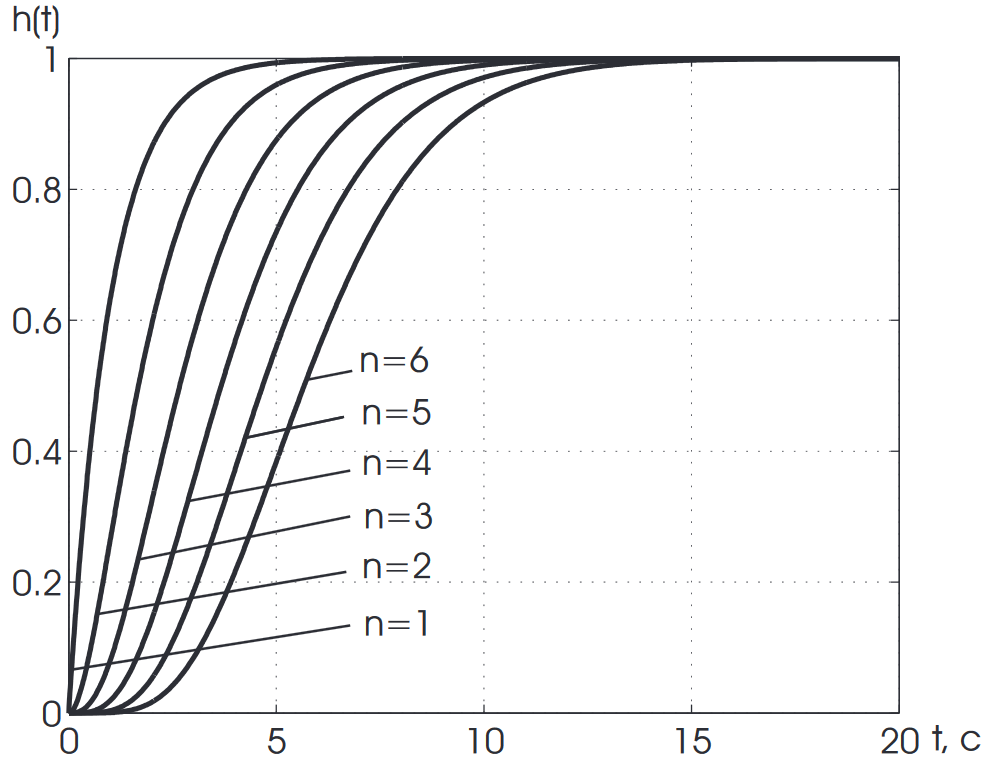
\includegraphics[height = 6cm]{img/newph.png}}
	\caption{Нормированные переходные характеристики полинома Ньютона}
	\label{newgraph}
\end{figure}

Такие корни характеристического полинома в теории обеспечивают апериодический характер переходных процессов, то есть с нулевым перерегулированием, однако в реальных системах управления достижение нулевого значения перерегулирования является весьма сложной задачей. Во многих случаях в системе присутствует перерегулирование, которое обусловлено инерционностью объекта управления.\\

Биномы Ньютоны с первого по третий порядок системы представлены в таблице:
\begin{center}
\begin{tabular}{ |c|c| } 
 \hline
 Порядок системы &  Стандартный полином Ньютона \\ 
 \hline
 1 & $\lambda+\omega_0$ \\ 
 \hline
 2 & $\lambda^2+2\omega_0\lambda+\omega_0^2$ \\ 
 \hline
 3 & $\lambda^3+3\omega_0\lambda^2+3\omega_0^2\lambda+\omega_0^3$ \\ 
 \hline
\end{tabular}\\
\end{center}

Соответственно, для системы \eqref{pidfunc} с характеристическим полиномом 3-го порядка можно записать:
\begin{equation}
	J_ms^3+(K+k_d)s^2+k_ps+k_i = s^3+\frac{(K+k_d)s^2}{J_m}+\frac{k_ps}{J_m} +\frac{k_i}{J_m} =(s+\omega_0)^3= s^3+3\omega_0s^2+3\omega_0^2s+\omega_0^3,
\end{equation}
откуда можно получить желаемые значения коэффициентов регулятора:
\begin{equation}
	k_p = 3\omega_0^2J_m, \phantom{- }k_i = \omega_0^3J_m, \phantom{- } k_d=3\omega_0J_m - K
\end{equation}

Аналогично для системы \eqref{pifunc}:
\begin{equation}
	J_ms^2+(K+k_p^1)s+k_i^1 = s^2+\frac{(K+k_p^1)s}{J_m}+\frac{k_i^1}{J_m} =(s+\omega_0)^2= s^2+2\omega_0s+\omega_0^2,
\end{equation}
откуда:
\begin{equation}
	k_p^1 = 2\omega_0J_m-k, \phantom{- }k_i^1 = \omega_0^2J_m
\end{equation}

Для формирования полинома Ньютона необходимо знать значение параметра $\omega_0$.  Определить этот параметр позволяет метод стандартных переходных функций основанный на нормированных переходных функциях. Нормированные переходные функции имеет только полюса, получаются путем замены значения параметра $\omega_0$ на единицу в формулах, определяющих полином Ньютона, и имеют вид:
%Проверь мысли свои как формулируешь
\begin{equation}
	W(s) = \frac{1}{D^*(s)}, \phantom{-} \omega_0=1
\end{equation}

Графики нормированных переходных функций, получаемые при подаче единичного воздействия на вход системы, для случая бинома Ньютона представлены на рис.~\ref{newgraph}

\begin{figure}[h]
	\noindent\centering{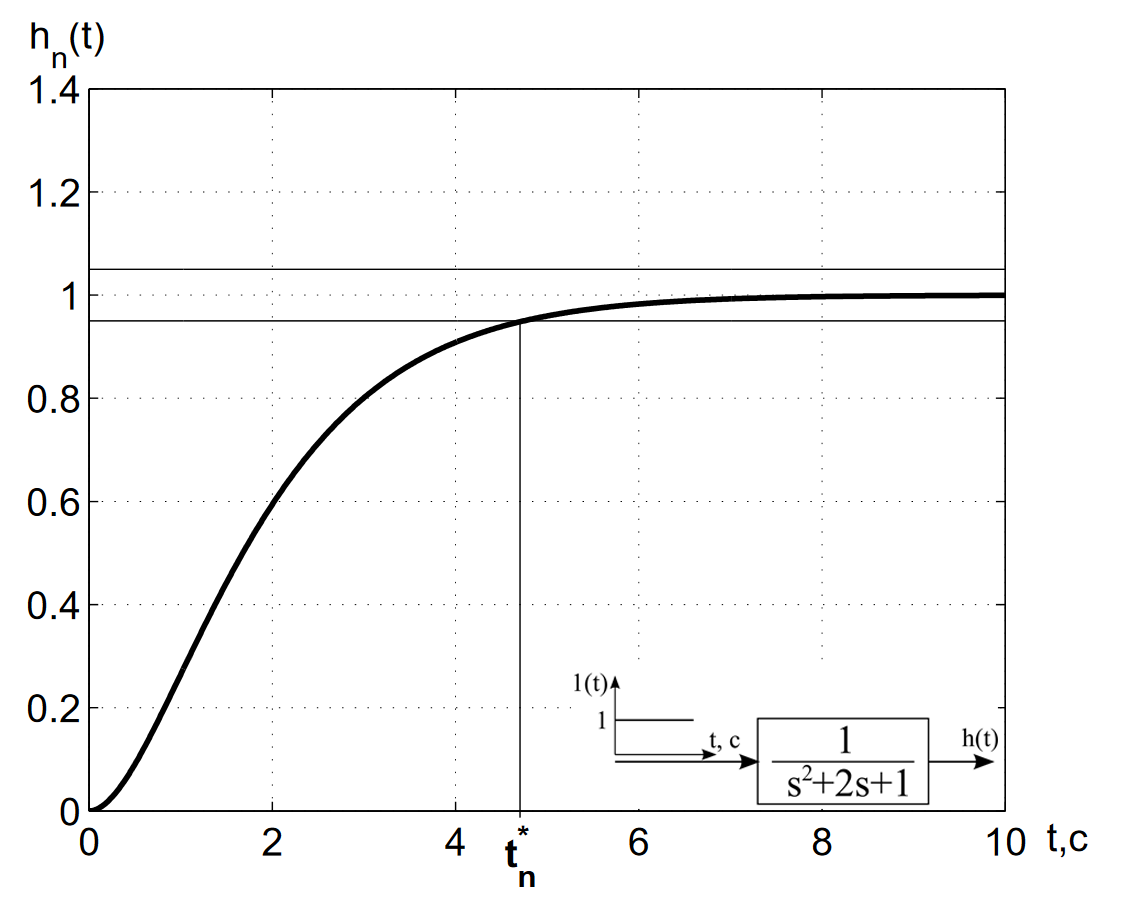
\includegraphics[height = 6cm]{img/newtime.png}}
	\caption{Определение времени переходного процесса }
	\label{newtime}
\end{figure}

Для нахождения требуемого характеристического полинома нужно определить время переходного процесса $t_n^*$, то есть определение момента времени, когда переходный процесс попадает в $\Delta$-область и больше её не покидает, где $\Delta$-область находится в приделах от 0,01\% до 0,05\% от установившегося значения переходного процесса. Нахождение  $t_n^*$ изображено на рис.~\ref{newtime}.

В таблице приведены $t_n^*$ для биномов Ньютона с 1-й по 3-й порядок:
\begin{center}
\begin{tabular}{ |c|c|c|c| } 
 \hline
 n &  1 & 2 & 3  \\ 
 \hline
 $t_n^*, c$ &  3.0 & 4.8 & 6.3  \\ 
 \hline
 $\sigma, \%$ &  0 & 0 & 0  \\ 
 \hline
\end{tabular}
\end{center}
где $\sigma$ - процент перерегулирования. 

Зная $t_n^*$ , на основе данного в техническом задании времени переходного процесса $t_n$, $\omega_0$ находится по формуле: 
\begin{equation}\label{omeganul}
	\omega_0=\frac{t_n^*}{t_n},
\end{equation}
основанной на принципе подобия, состоящего в том, что увеличение параметра $\omega_0$ приводит к увеличению скорости протекания процессов в системе, но при этом не оказывает влияния на колебательность этих процессов.

Результаты моделирования систем \eqref{pidfunc} и \eqref{pifunc} с коэффициентами, полученными из бинома Ньютона изображены на рис.~\ref{pidmod} и рис.~\ref{pimod} соответственно.

\begin{figure}[h]
	\noindent\centering{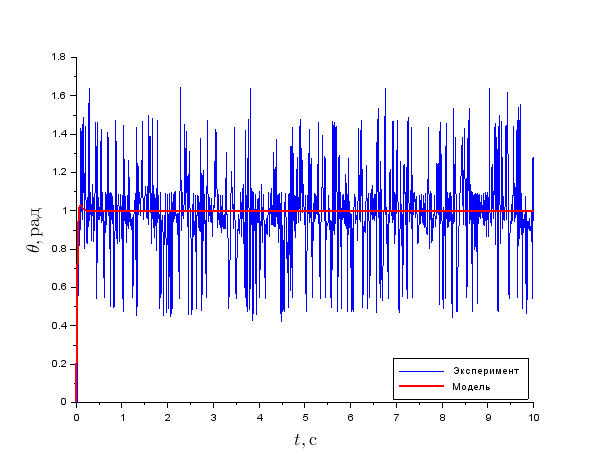
\includegraphics[height = 6cm]{img/N1.png}}
	\caption{График ПИД-регулятора с коэффициентами, полученными из бинома Ньютона при времени переходного процесса 0.1 сек }
	\label{pidmod}
\end{figure}

\begin{figure}[h]
	\noindent\centering{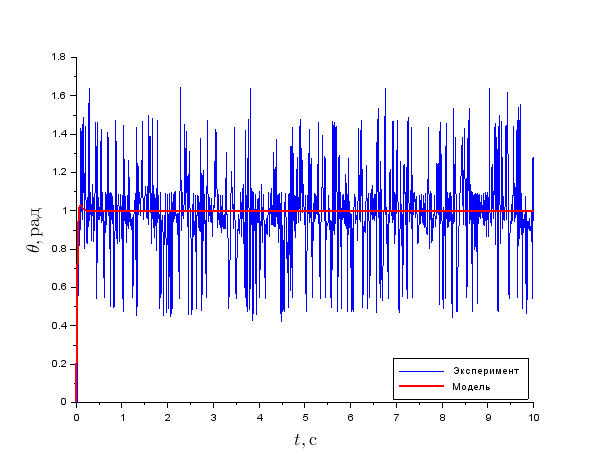
\includegraphics[height = 6cm]{img/N1.png}}
	\caption{График ПИ-регулятора с коэффициентами, полученными из бинома Ньютона при времени переходного процесса 0.1 сек }
	\label{pimod}
\end{figure}

\paragraph*{Полином Баттерворта\\}
\hspace*{\parindent}Еще одним полиномом, применяемым для нахождения коэффициентов, является полином Баттерворта, выражаемый следующим образом: 
\begin{equation}
	D^*(\lambda)=\prod_{i=1}^{n}(\lambda-\lambda_i^*).
\end{equation}
Его корни расположены в левой полуплоскости $s$ на полуокружности с радиусом $\omega_0$ и находятся по формуле:
\begin{equation}
	\lambda_i^*=\omega_0(\cos{\frac{\pi(2i-1)}{n}}+j\sin{\frac{\pi(2i-1)}{n}}),\phantom{-}i=\overline{1,n}.
\end{equation}\begin{figure}[h]
	\noindent\centering{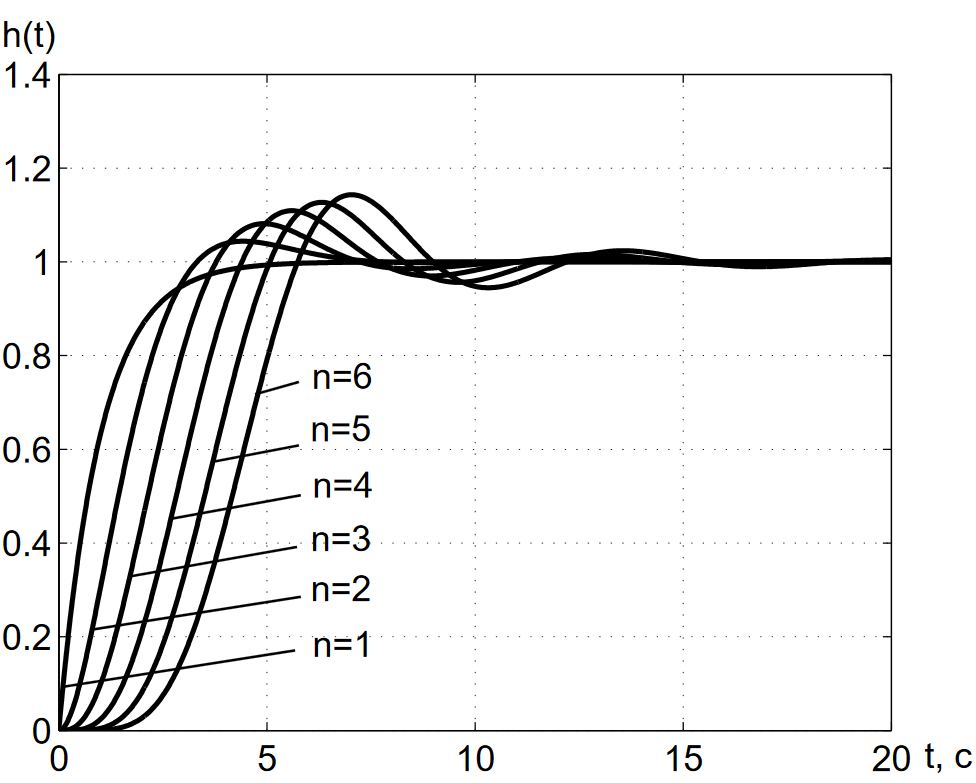
\includegraphics[height = 6cm]{img/buttergraph.png}}
	\caption{Нормированные переходные характеристики полинома Баттерворта}
	\label{buttergraph}
\end{figure}

Полиномы Баттерворта с первого по третий порядок системы представлены в таблице:
\begin{center}
\begin{tabular}{ |c|c| } 
 \hline
 Порядок системы &  Стандартный полином Баттерворта \\ 
 \hline
 1 & $\lambda+\omega_0$ \\ 
 \hline
 2 & $\lambda^2+1.4\omega_0\lambda+\omega_0^2$ \\ 
 \hline
 3 & $\lambda^3+2\omega_0\lambda^2+2\omega_0^2\lambda+\omega_0^3$ \\ 
 \hline
\end{tabular}
\end{center}

Коэффициенты системы находятся по такому же принципу, как и в случае с биномом Ньютона:
\begin{equation}
	J_ms^3+(K+k_d)s^2+k_ps+k_i = s^3+\frac{(K+k_d)s^2}{J_m}+\frac{k_ps}{J_m} +\frac{k_i}{J_m} =(s+\omega_0)^3= s^3+2\omega_0s^2+2\omega_0^2s+\omega_0^3,
\end{equation}
\begin{equation}
	k_p = 2\omega_0^2J_m, \phantom{- }k_i = \omega_0^3J_m, \phantom{- } k_d=2\omega_0J_m - K
\end{equation}
\begin{equation}
	J_ms^2+(K+k_p^1)s+k_i^1 = s^2+\frac{(K+k_p^1)s}{J_m}+\frac{k_i^1}{J_m} = s^2+1.4\omega_0s+\omega_0^2,
\end{equation}
\begin{equation}
	k_p^1 =1.4\omega_0J_m-K, \phantom{- }k_i^1 = \omega_0^2J_m
\end{equation}

Коэффициент $\omega_0$ находится по формуле \eqref{omeganul}

Из графиков нормированных функций полинома Баттерворта на рис. \ref{buttergraph} видно, что перерегулирование составляет меньше 20\%.

В таблице приведены $t_n^*$ для полиномов Баттерворта с 1-й по 3-й порядок:
\begin{center}
\begin{tabular}{ |c|c|c|c| } 
 \hline
 n &  1 & 2 & 3  \\ 
 \hline
 $t_n^*, c$ &  3.0 & 2.9 & 6.0  \\ 
 \hline
 $\sigma, \%$ &  0.0 & 4.5 & 8  \\ 
 \hline
\end{tabular}
\end{center}
где $\sigma$ - процент перерегулирования. 

Результаты моделирования систем \eqref{pidfunc} и \eqref{pifunc} с коэффициентами, полученными из полинома Баттерворта изображены на рис.~\ref{pidmod2} и рис.~\ref{pimod2} соответственно.

\begin{figure}[h]
	\noindent\centering{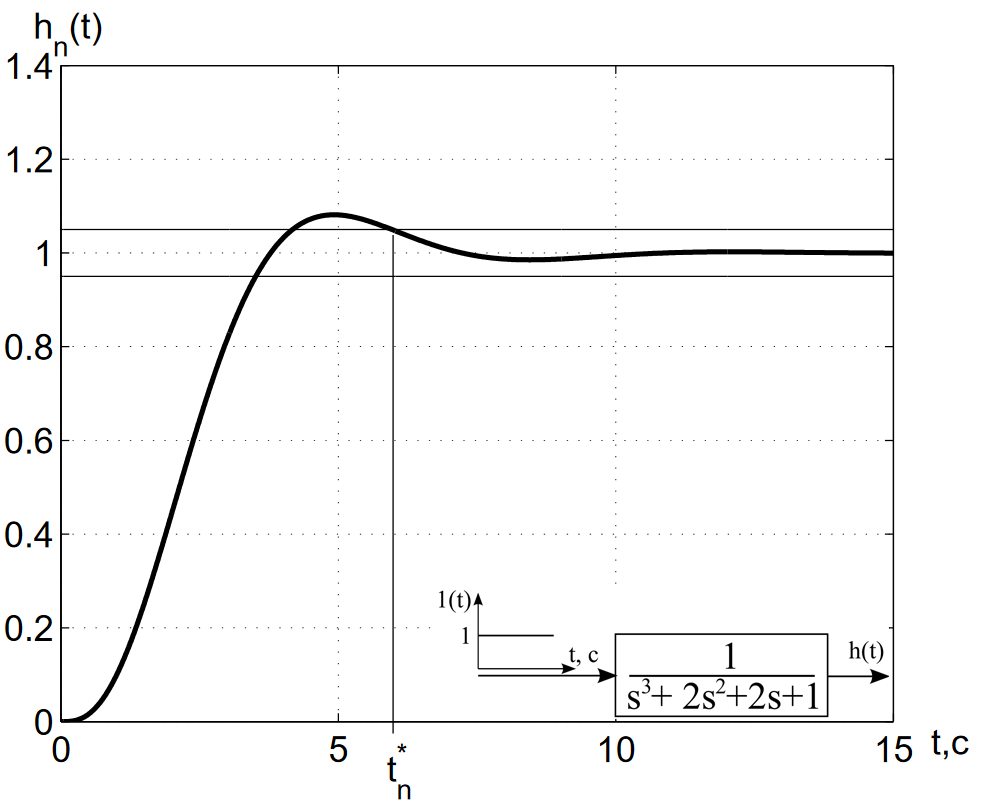
\includegraphics[height = 6cm]{img/buttertime.png}}
	\caption{Определение времени переходного процесса }
	\label{buttertime}
\end{figure}

\begin{figure}[h]
	\noindent\centering{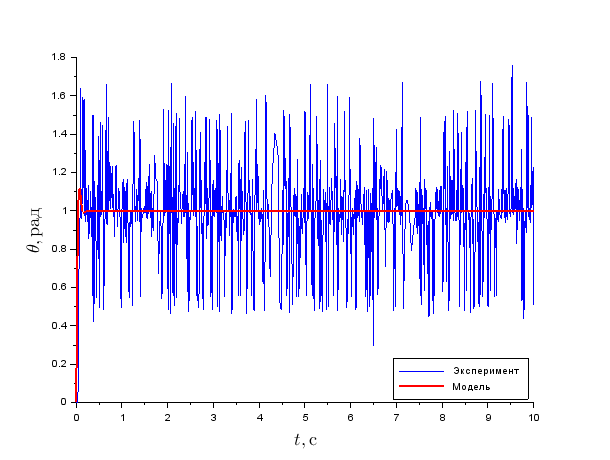
\includegraphics[height = 6cm]{img/B05.png}}
	\caption{График ПИД-регулятора с коэффициентами, полученными из полинома Баттерворта при времени переходного процесса 0.05 сек }
	\label{pidmod2}
\end{figure}

\begin{figure}[h]
	\noindent\centering{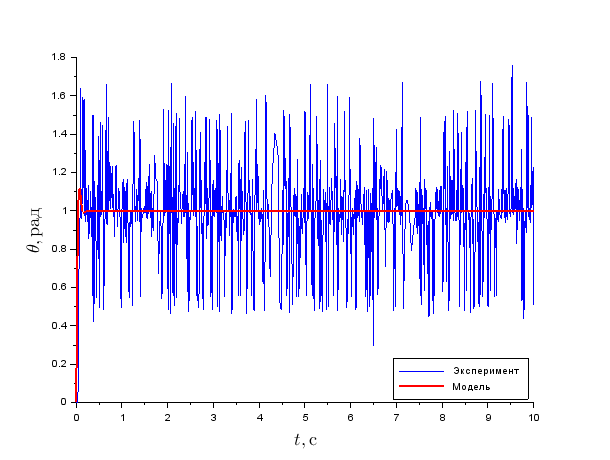
\includegraphics[height = 6cm]{img/B05.png}}
	\caption{График ПИ-регулятора с коэффициентами, полученными из полинома Баттерворта при времени переходного процесса 0.05 сек }
	\label{pimod2}
\end{figure}

\end{document}